\documentclass[12pt]{article}  % standard LaTeX, 12 point type
\usepackage{amsfonts,latexsym}
\usepackage{amsthm}
\usepackage{amssymb}
\usepackage[utf8x]{inputenc} % Кодировка
\usepackage[english]{babel} % Многоязычность
\usepackage{amsmath}
\usepackage{tikz}
\usetikzlibrary{automata,positioning}

\usepackage{algpseudocode}
\usepackage{algorithm}
\usepackage{caption}
\usepackage{algorithmicx}


\newtheorem{theorem}{Theorem}[section]
\newtheorem{proposition}[theorem]{Proposition}
\newtheorem{lemma}[theorem]{Lemma}
\newtheorem{corollary}[theorem]{Corollary}
\newtheorem{conjecture}[theorem]{Conjecture}

\theoremstyle{definition}
\newtheorem{definition}{Определение}[section]
\newtheorem{example}{Example}[section]

% unnumbered environments:

\theoremstyle{remark}
\newtheorem*{remark}{Remark}
\newtheorem*{notation}{Notation}
\newtheorem*{note}{Note}

\setlength{\parskip}{5pt plus 2pt minus 1pt}
%\setlength{\parindent}{0pt}

\usepackage{color}
\usepackage{listings}
\usepackage{caption}
\usepackage{graphicx}
\usepackage{ucs}

\newcommand{\tab}[1][0.3cm]{\ensuremath{\hspace*{#1}}}
% A generalized view on parsing and translation
% http://dl.acm.org/citation.cfm?id=2206331
\title{Rytter for CFPQ}
% Context-free path querying ...
\author{Semyon Grigorev
\\
       {Saint Petersburg State University}\\
       {7/9 Universitetskaya nab.}\\
       {St. Petersburg, 199034, Russia}\\
       semen.grigorev@jetbrains.com, rsdpisuy@gmail.com
       }
\author{Ekaterina Shemetova
\\
       {University}\\
       {u1}\\
       {u2}\\
       e-mail@edu-domain
       }
\date{\today}

\date{}


\begin{document}

\algtext*{EndWhile}% Remove "end while" text
\algtext*{EndIf}% Remove "end if" text
\algtext*{EndFor}% Remove "end for" text
\algtext*{EndFunction}% Remove "end function" text

\maketitle
\section {Linear input}

Let the input grammar is 
\begin{align*}
S & \rightarrow a \ S \ b \ 
\\
S & \rightarrow S \ S
\\
S & \rightarrow a \ b
\end{align*}


The input grammar in CNF is 
\begin{align*}
S   & \rightarrow A \ S_1
\\
S_1 & \rightarrow S \ B
\\
S & \rightarrow S \ S
\\
S   & \rightarrow A \ B
\\
A   & \rightarrow a
\\
B   & \rightarrow b
\end{align*}

Input: $abab$

Grid:
\\
\begin{tikzpicture}[shorten >=1pt,node distance=4cm,on grid,auto] 
   \node[state] (q_1)   {$1$}; 
   \node[state] (q_2) [right=of q_1] {$2$}; 
   \node[state] (q_3) [right=of q_2] {$3$}; 
   \node[state] (q_4) [right=of q_3] {$4$};

   \node[state] (q_5) [below=of q_1] {$5$};
   \node[state] (q_6) [right=of q_5] {$6$};
   \node[state] (q_7) [right=of q_6] {$7$};
   \node[state] (q_8) [right=of q_7] {$8$};
  
   \node[state] (q_9) [below=of q_5] {$9$};
   \node[state] (q_10) [right=of q_9] {$10$};
   \node[state] (q_11) [right=of q_10] {$11$};
   \node[state] (q_12) [right=of q_11] {$12$};
   
   \node[state] (q_13) [below=of q_9] {$13$};
   \node[state] (q_14) [right=of q_13] {$14$};
   \node[state] (q_15) [right=of q_14] {$15$};
   \node[state] (q_16) [right=of q_15] {$16$};

    \path[->] 
    (q_2) edge[bend left]  node {$S_1$} (q_4)          
    (q_1) edge[bend left]  node {$S_2$} (q_4)          
    (q_9) edge  node {$S$} (q_5)
    (q_10) edge  node {$S$} (q_6);
\end{tikzpicture}


\section {Graph input} 

Let the input grammar is 
\begin{align*}
S & \rightarrow a \ S \ b \ 
\\
S & \rightarrow a \ b
\end{align*}


The input grammar in CNF is 
\begin{align*}
S   & \rightarrow A \ S_1
\\
S_1 & \rightarrow S \ B
\\
S   & \rightarrow A \ B
\\
A   & \rightarrow a
\\
B   & \rightarrow b
\end{align*}


Let the input graph is
\\
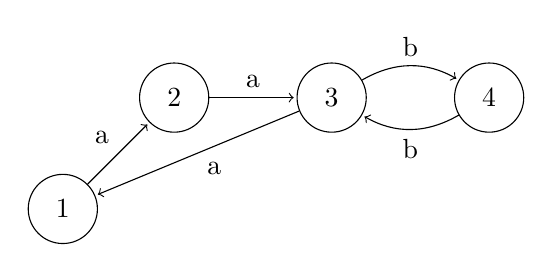
\begin{tikzpicture}[shorten >=1pt,node distance=2cm,on grid,auto] 
   \node[state] (q_1)   {$1$}; 
   \node[state] (q_2) [above right=of q_1] {$2$}; 
   \node[state] (q_3) [right=of q_2] {$3$}; 
   \node[state] (q_4) [right=of q_3] {$4$};
    \path[->] 
    (q_1) edge  node {a} (q_2)          
    (q_2) edge  node {a} (q_3)
    (q_3) edge  node {a} (q_1)
    (q_3) edge[bend left, above]  node {b} (q_4)
    (q_4) edge[bend left, below]  node {b} (q_3);
\end{tikzpicture}

Grid:
\\
\begin{tikzpicture}[shorten >=1pt,node distance=4cm,on grid,auto] 
   \node[state] (q_1)   {$1$}; 
   \node[state] (q_2) [right=of q_1] {$2$}; 
   \node[state] (q_3) [right=of q_2] {$3$}; 
   \node[state] (q_4) [right=of q_3] {$4$};

   \node[state] (q_5) [below=of q_1] {$5$};
   \node[state] (q_6) [right=of q_5] {$6$};
   \node[state] (q_7) [right=of q_6] {$7$};
   \node[state] (q_8) [right=of q_7] {$8$};
  
   \node[state] (q_9) [below=of q_5] {$9$};
   \node[state] (q_10) [right=of q_9] {$10$};
   \node[state] (q_11) [right=of q_10] {$11$};
   \node[state] (q_12) [right=of q_11] {$12$};
   
   \node[state] (q_13) [below=of q_9] {$13$};
   \node[state] (q_14) [right=of q_13] {$14$};
   \node[state] (q_15) [right=of q_14] {$15$};
   \node[state] (q_16) [right=of q_15] {$16$};

    \path[->] 
    (q_2) edge[bend left]  node {$S_1$} (q_4)          
    (q_1) edge[bend left]  node {$S_2$} (q_4)          
    (q_9) edge  node {$S$} (q_5)
    (q_10) edge  node {$S$} (q_6);
\end{tikzpicture}


\
\begin{thebibliography}{9}

\bibitem{OptimalDLR}
Krishnendu Chatterjee, Bhavya Choudhary, and Andreas Pavlogiannis. 
2017. 
\emph{Optimal Dyck reachability for data-dependence and alias analysis.}
Proc. ACM Program. Lang. 2, POPL, Article 30 (December 2017), 30 pages. DOI: 
https://doi.org/10.1145/3158118


%\bibitem{ParsingWithPictures}
%  Keshav Pingali, and Gianfranco Bilardi. 
%  \emph{A Graphical Model for Context-Free Grammar Parsing.}
%   International Conference on Compiler Construction. Springer, Berlin, Heidelberg, 2015.


\end{thebibliography}


\end{document}